 \chapter{Background}
 \minitoc


 \section{Introduction}
 \label{sec:ch1_Introduction }
% In this chapter, we present the background necessary to appreciate our proposed combination of texture descriptors to recognise facial expression. We present a generic overview of several concepts in this chapter, while the specific usages of
%various techniques and associated rationale are described in related chapters.


 
 In this chapter, we present the background necessary to appreciate our proposed method based on image texture and r Random forest. We show a generic overview of various main concepts, with the more specific details of different techniques in relevant chapters. 
 
 Facial expression recognition field was first started being discussed at the end of the last century \citep{essa1995facial}. Since then, many researchers have proposed methods to improve the ability of machines to recognise human facial expressions.   

\section{Review of main classification emotions methods }
 
\subsection{Active shape model And  Active appearance model}
\label{sec:ch1_ASM}
An active appearance model (AAM) \citep{edwards1998interpreting, cootes1998activeApearance,cootes2001active} is a computer vision algorithm which depends on  statistically finding the values which fit with a grey image's texture values, and making a statistical link with an active shape model \citep{cootes1992active,cootes1992training,cootes1995active}.
ASM was first proposed by \citet{cootes1992active} based on models created from sets of training examples called Point Distribution Models (PDM), which represent objects as sets of labelled points called landmark points. Figure \ref{fig:PDM} illustrates a PDM as an example of face points landmarking. AAM was first proposed by \citet{edwards1998interpreting} for face analysis. Since then the method has been commonly used in computer vision applications such as face matching, tracking faces, medical image analysis and emotions recognition \citep{ratliff2008emotion,ko2010development,setyati2012facial,lozano2014facial,chen2013gc,yu2013pose}. 

The training set are normally labelled manually, each shape is represented as shown in equation \ref{equ:points}. The first step is computing the mean points for all the training set to find the mean shape $\boldsymbol{\bar{x}}$. 
%%%%%%%%%%%%%%%%%%%%%%%%%%%%%%%%%%%%%%%%%%%%%%%%%%%%%%%%%%%%%%%%%
\begin{equation}
\boldsymbol{x} = (x_0, y_0 , x_1, y_1,  ..., x_k, y_k, ..., x_{n-1}, y_{n-1})^T
    \label{equ:points}
\end{equation}
%%%%%%%%%%%%%%%%%%%%%%%%%%%%%%%%%%%%%%%%%%%%%%%%%%%%%%%%%%%%%%%%%
where $ (x_k, y_k$)is the position point $k$ 

AAM's idea is to combine a model of face shape variation with a model of the appearance variations of a shape-normalised face.
 To create new shapes from the mean shape $\boldsymbol{\bar{x}}$, ASM variates new shapes and textures using Principal Component Analysis (PCA). PCA is applied to all training data to calculate the eigenvectors of the covariance matrix. To generate a new shape, the following equation is used:
%%%%%%%%%%%%%%%%%%%%%%%%%%%%%%%%%%%%%%%%%%%%%%%%%%%%%%%%%%%%%%%%%
\begin{equation}
\boldsymbol{x} \approx \boldsymbol{\bar{x}} + \boldsymbol{P}_s \boldsymbol{b}_s
    \label{equ:NewShapes}
\end{equation}
%%%%%%%%%%%%%%%%%%%%%%%%%%%%%%%%%%%%%%%%%%%%%%%%%%%%%%%%%%%%%%%%%
where $\boldsymbol{\bar{x}}$ the mean shape, $\boldsymbol{P}= (\boldsymbol{P}_1 \mid \boldsymbol{P}_2\mid...\mid \boldsymbol{P}_t)$  contains t eigenvectors of the covariance matrix and $\boldsymbol{b}$ is a t dimensional vector given by

%%%%%%%%%%%%%%%%%%%%%%%%%%%%%%%%%%%%%%%%%%%%%%%%%%%%%%%%%%%%%%%%
\begin{equation}
\boldsymbol{b} = \boldsymbol{P}^T (\boldsymbol{x-\bar{x}})
    \label{equ:points}
\end{equation}
%%%%%%%%%%%%%%%%%%%%%%%%%%%%%%%%%%%%%%%%%%%%%%%%%%%%%%%%%%%%%%%%%
 
 All image shapes are normalised to the mean shape; then each image is warped to its control points. The same pose (translation, scale and rotation) values are used in shape normalisation so that we can sample the grey level information $\boldsymbol{g}$ from a shape-normalised face patch. By applying PCA to this data we obtain this model:
 

%%%%%%%%%%%%%%%%%%%%%%%%%%%%%%%%%%%%%%%%%%%%%%%%%%%%%%%%%%%%%%%%
\begin{equation}
\boldsymbol{g} \approx \boldsymbol{\bar{g}} + \boldsymbol{P}_g \boldsymbol{b}_g
    \label{equ:NewGreys}
\end{equation}
%%%%%%%%%%%%%%%%%%%%%%%%%%%%%%%%%%%%%%%%%%%%%%%%%%%%%%%%%%%%%%%%%

A further PCA is applied to correlated shape and grey-level variations, to obtain:

\begin{equation}
\boldsymbol{x} \approx \boldsymbol{\bar{x}} + \boldsymbol{Q}_s \boldsymbol{c}
    \label{equ:ModelNewShapes}
\end{equation}

\begin{equation}
\boldsymbol{g} \approx \boldsymbol{\bar{g}} + \boldsymbol{Q}_g \boldsymbol{c}
    \label{equ:ModelNewShapes}
\end{equation}

where $\boldsymbol{\bar{x}}$.  is the mean shape, $\boldsymbol{\bar{g}}$.  the mean texture, $Q_s,Q_g$ are matrices describing the
modes of variation derived from the training set and $c$ are the model parameters.

By varying the elements of $\boldsymbol{c}$ in equation \ref{equ:ModelNewShapes} and \ref{equ:NewGreys}, new shapes and images will be generated. So $c_i$ is the variance of the $i_{th}$  parameter given by  $ \lambda_i$. To generate similar shapes to the original training data, limits of $\pm3 \sqrt[]{\lambda_i}$ have been applied to the parameter $b_i$. 

Now if we were given a new image $g_s$, and we want to find the shape points which fit the image we need to vary $\boldsymbol{c}$ to generate new images by a set of model parameters, c, we can generate a hypothesis
for the shape, $x$, and texture, $g_m$, of a model instance, then finding the most similar generated image for the appearance model to $g_s$ by computing the
difference, $\delta g = g_s - g_m$.  This is an optimisation problem to find the best $\boldsymbol{c}$ efficiently, which will generate shape landmarks which describe the face parts.




%%%%%%%%%%%%%%%%%%%%%%%%%%%%%%%%%%%%%%%%%%%%%%%%%%%%%%%%%%%%%%%%%
\begin{figure}[H]
\centering
  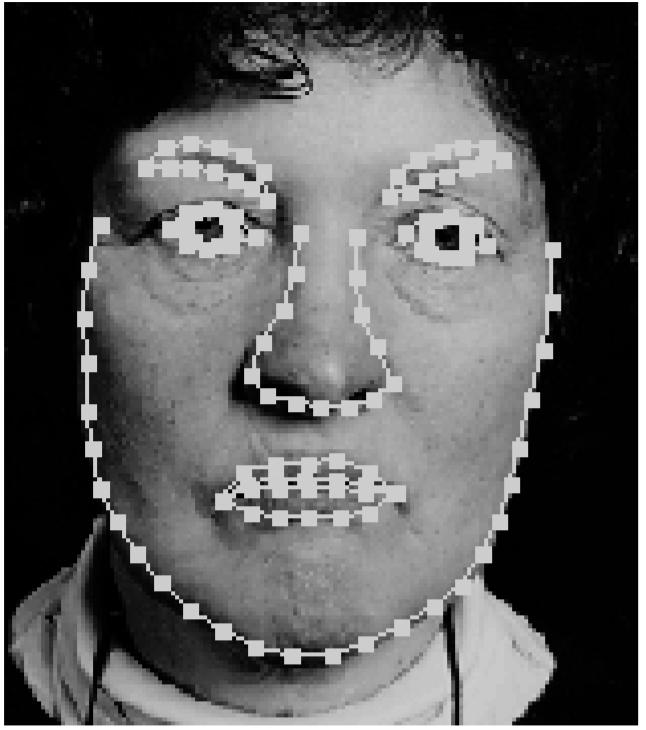
\includegraphics[width=0.3\textwidth]{Chapter2/Figs/FacePoints.png}
  \textbf{
    \caption{Point Distribution Model \citep{cootes1999comparing}}
    \label{fig:PDM}}
\end{figure}
%%%%%%%%%%%%%%%%%%%%%%%%%%%%%%%%%%%%%%%%%%%%%%%%%%%%%%%%%%%%%%%%%



Since \citet{edwards1998interpreting}, many researches have used AAM in many applications to  recognise facial expression in f videos \cite{sung2006real, martin2008real} and photos \cite{kanade2000comprehensive, van2005model,wu2013facial} . Facial expressions recognition is one the most discussed topics during the last three decades. Researchers have applied AAM to extract facial features face points to be classified using various classifiers. One of the ways that AAM has been used in facial recognition system is to detect action units as described in the Facial Action Coding System (FACS) \cite{ekman1978facial}, which was based on minimal muscular movements  and which individually or in combinations  represents all facial expressions \citep{cohn1998feature, van2005model,lucey2010extended} By finding  the action units existing in a face , and by using one or a group of them together, facial expression can be recognised. For an instance, AU1 is Inner Brow Raiser, AU2 is Outer Brow Raiser, AU15 Lip Corner Depressor and AU28 Lip Suck. To determine anger expression, for example, AU23 and AU24 must be present in the AU combination, where AU1+4+15 or 11 must be present for sadness \cite{lucey2010extended}. 
To classify the extracted features to find the AUs trained classifiers have been used like neural networks trained with back propagation \citet{van2005model} on Cohn-Kanade AU-Coded (CK+) Facial Expression Database \citet{kanade2000comprehensive}, or Support Vector Machine (SVM) in \citet{lucey2010extended} with (CK+) database as well.     

On the other hand, AAM was used to detect the facial expressions directly rather than AUs detection. The AAM features have been classified with several classifiers such as simple Euclidean-distance classification scheme \cite{ratliff2008emotion},  K-means classification \cite{martins2008facial} or SVM \citet{pu2015facial}.






\subsection{Image texture based methods}
\label{sec:ch1_Imagetexture}
Image texture based or appearance-based methods have been widely used in computer vision applications face recognition and facial expressions recognition. The idea of image texture methods is using the image pixel values such as RGB, grey scale changes or illumination. Many methods have been proposed to describe the image and extract the image features such as Locally Binary Patterns(LBP), Histogram of oriented gradients (HOG) scale-invariant feature transform (SIFT) and speeded up robust features (SURF).






%__________________________________________________________HOG__________________________________________________________________
%__________________________________________________________HOG__________________________________________________________________
%__________________________________________________________HOG__________________________________________________________________

\subsubsection{Local histogram of oriented gradients (HOG)}

Local histogram of oriented gradients (HOG) is a method proposed by Dalal et al.\citep{dalal2005histograms}. This method aims to describe an image with a set of local histograms. These histograms count occurrences of gradient orientation in a local part of the image. The HOG algorithm is similar to edge orientation histograms, scale-invariant feature transform descriptors, and shape contexts, but differs in that it is computed on a dense grid of uniformly spaced cells and uses overlapping local contrast normalisation for improved accuracy\citep{dalal2005histograms}. Figure \ref{fig:HOGVisual} shows a HOG feature visualization for a face. By focusing on the image, you can see the basic features of the image.

There are several primary steps for extracting HOG features: the first is Gamma/Colour Normalisation, where \citet{dalal2005histograms} found that gamma normalisation improves the classification rate. It is important to know that gamma normalisation gives a minor improvement so we can skip the step. The second step is computing the image gradients by applying the 1-D centred. Dalal and Triggs found that this gives the best results in one or both of the horizontal and vertical directions, $ [-1,0,1] $ for vertical and $ [-1,0,1] ^T$ for horizontal.
At every pixel we calculate a value for the x-derivative and another value for the y-derivative for x and y gradient magnitudes respectively, let us call them $Sx$ and $Sy$. The equations defining the gradients are, respectively being:


%%%%%%%%%%%%%%%%%%%%%%%%%%%%%%%%%%%%%%%%%%%%%%%%%%%%%%%%%%%%%%%%%
\begin{equation}\label{eq:HOG1}
S_x (i,j) = \frac{\partial I}{\partial x} (i,j)
\end{equation}
%%%%%%%%%%%%%%%%%%%%%%%%%%%%%%%%%%%%%%%%%%%%%%%%%%%%%%%%%%%%%%%%%

%%%%%%%%%%%%%%%%%%%%%%%%%%%%%%%%%%%%%%%%%%%%%%%%%%%%%%%%%%%%%%%%
\begin{equation}\label{eq:HOG2}
S_y (i,j) = \frac{\partial I}{\partial y} (i,j)
\end{equation}
%%%%%%%%%%%%%%%%%%%%%%%%%%%%%%%%%%%%%%%%%%%%%%%%%%%%%%%%%%%%%%%%%

where $I$ is an image, and $(i, j)$ the pixel coordinates.

The gradient magnitude itself $M$ is computed as the square root of the quadratic sum of each gradient component, this is:
%%%%%%%%%%%%%%%%%%%%%%%%%%%%%%%%%%%%%%%%%%%%%%%%%%%%%%%%%%%%%%%%%
\begin{equation}\label{eq:HOG3}
M(i,j) = \sqrt[]{S_x^2(i,j) + S_y^2(i,j)}
\end{equation}
%%%%%%%%%%%%%%%%%%%%%%%%%%%%%%%%%%%%%%%%%%%%%%%%%%%%%%%%%%%%%%%%%
The gradient orientation angle is calculated by: 
%%%%%%%%%%%%%%%%%%%%%%%%%%%%%%%%%%%%%%%%%%%%%%%%%%%%%%%%%%%%%%%%%
\begin{equation}\label{eq:HOG4}
\theta (i,j) = arctan \left(\frac{S_x(i,j)}{S_y(i,j)} \right)
\end{equation}
%%%%%%%%%%%%%%%%%%%%%%%%%%%%%%%%%%%%%%%%%%%%%%%%%%%%%%%%%%%%%%%%%

The third step is called Orientation Binning which aims to build a histogram of orientation for each cell; ( where the image was subdivided into little cells). 
Each pixel within the cell gives a weighted vote for an orientation-based histogram channel based on the values found in the gradient results. This histograms represent
angles evenly spaced between \ang{0} and \ang{180} (“unsigned” gradient) or within \ang{0} and \ang{-360} (“signed” gradient). 


%%%%%%%%%%%%%%%%%%%%%%%%%%%%%%%%%%%%%%%%%%%%%%%%%%%%%%%%%%%%%%%%%
\begin{figure}[H]
\centering
  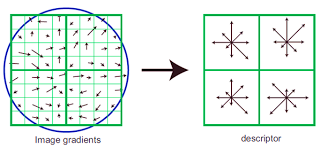
\includegraphics[width=0.4\textwidth]{Chapter4/Figs/gradients_and_binning.png}
  \textbf{
    \caption{ Image Gradients and Spatial/Orientation Binning.}
    \label{fig:GradientsBinning}}
\end{figure}
%%%%%%%%%%%%%%%%%%%%%%%%%%%%%%%%%%%%%%%%%%%%%%%%%%%%%%%%%%%%%%%%%


The final step is block normalising histograms within each block of cells. Because of gradient strength variation as a result of local  illumination variations and the foreground-background contrast, \citet{dalal2005histograms} found that some illumination normalization must be done to be essential for better accuracy. They explored different normalization schemes to achieve that. Let us define first $v$ as the vector containing all the histograms for a given block, $\|v\|_k$ the k-norm of $v$ with $k\in 1,2$ and let $\epsilon$  be a small constant. The normalization schemes are:

%%%%%%%%%%%%%%%%%%%%%%%%%%%%%%%%%%%%%%%%%%%%%%%%%%%%%%%%%%%%%%%%%
\begin{equation}\label{eq:L1-norm}
L1-norm: v\rightarrow \frac{v}{    \|v\|_2 + \epsilon}
\end{equation}
%%%%%%%%%%%%%%%%%%%%%%%%%%%%%%%%%%%%%%%%%%%%%%%%%%%%%%%%%%%%%%%%%

%%%%%%%%%%%%%%%%%%%%%%%%%%%%%%%%%%%%%%%%%%%%%%%%%%%%%%%%%%%%%%%%%
\begin{equation}\label{eq:L1-squared}
L1-squared norm: v\rightarrow \sqrt[]{\frac{v}{    \|v\|_2 + \epsilon}}
\end{equation}
%%%%%%%%%%%%%%%%%%%%%%%%%%%%%%%%%%%%%%%%%%%%%%%%%%%%%%%%%%%%%%%%%

%%%%%%%%%%%%%%%%%%%%%%%%%%%%%%%%%%%%%%%%%%%%%%%%%%%%%%%%%%%%%%%%%
\begin{equation}\label{eq:L2-norm}
L2-norm: v\rightarrow \frac{v}{\sqrt[]{    \|v\|_2^2 + \epsilon^2}}
\end{equation}
%%%%%%%%%%%%%%%%%%%%%%%%%%%%%%%%%%%%%%%%%%%%%%%%%%%%%%%%%%%%%%%%%

Dalal and Triggs' experiments found that L1-norm-squared and L2-norm performs similarly and achieves good results, but L1-norm decreases performance in a 5\%. Not normalizing reduces enormously the performance by around 27\%. 


%%%%%%%%%%%%%%%%%%%%%%%%%%%%%%%%%%%%%%%%%%%%%%%%%%%%%%%%%%%%%%%%%%
%\begin{equation}\label{eq:NoOfLBPCells}
%h_k
%\end{equation}
%%%%%%%%%%%%%%%%%%%%%%%%%%%%%%%%%%%%%%%%%%%%%%%%%%%%%%%%%%%%%%%%%%





\begin{figure}
\centering
\begin{subfigure}{.5\textwidth}
  \centering
  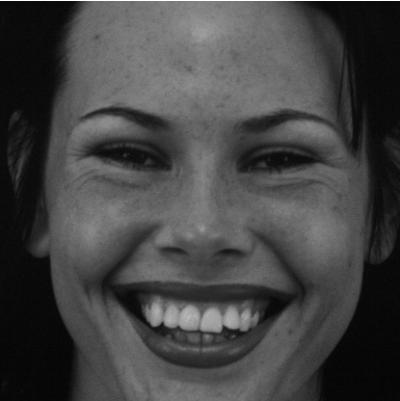
\includegraphics[width=.7\linewidth]{Chapter4/Figs/FaceHOG.png}
  \caption{A woman's face}
  \label{fig:sub1}
\end{subfigure}%
\begin{subfigure}{.5\textwidth}
  \centering
  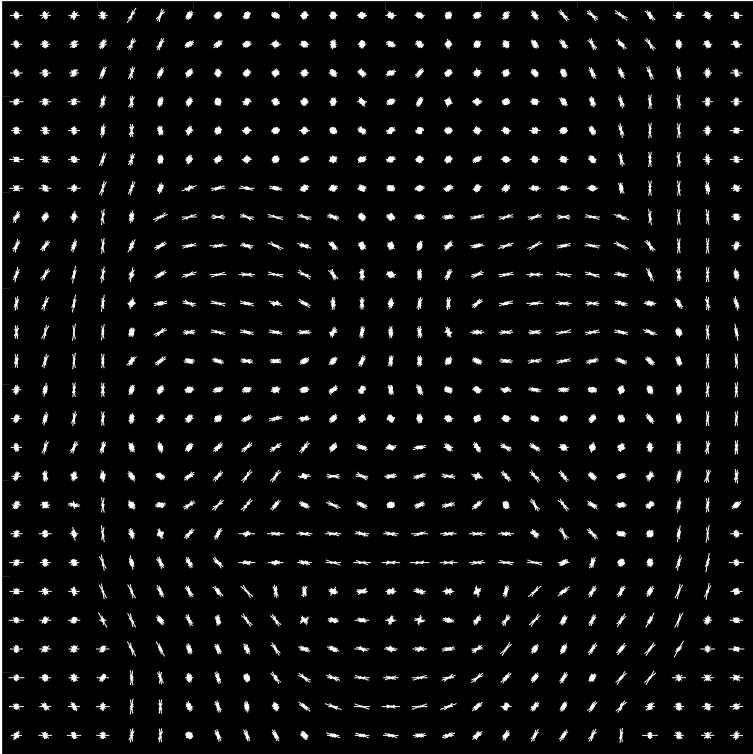
\includegraphics[width=.7\linewidth]{Chapter4/Figs/HOG.png}
  \caption{Visualization of extracted HOG }
  \label{fig:sub2}
\end{subfigure}
\caption{HOG descriptor Visualization}
\label{fig:HOGVisual}
\end{figure}



HOG method has been wildly used in computer vision to recognise objects. HOG features have used in facial expression recognition with multi-class RBF-SVM by extracting dense grid-based HOG features from images \citep{dahmane2011emotion}, where they used a cropped region from the aligned face and  divided it into (48) squares 8 rows and 6 columns. In \citet{dahmane2011emotion}, GEMEP-FERA dataset was used for training and testing 5 facial expressions anger, fear, joy, relief and sadness. The face has been divided into its main parts then extract each part's HOG features as shown in figure \ref{fig:HOGSyst}.


%%%%%%%%%%%%%%%%%%%%%%%%%%%%%%%%%%%%%%%%%%%%%%%%%%%%%%%%%%%%%%%%%
\begin{figure}[H]
\centering
  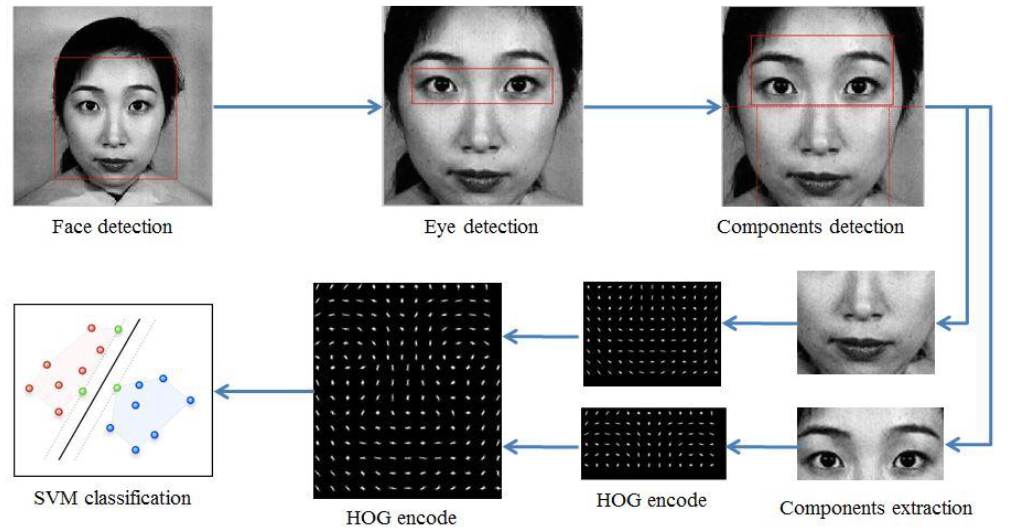
\includegraphics[width=0.65\textwidth]{Chapter2/Figs/HOGSyst.png}
  \textbf{
    \caption{An overview of the face recognition system with HOG \citep{chen2014facial}}
    \label{fig:HOGSyst}}
\end{figure}
%%%%%%%%%%%%%%%%%%%%%%%%%%%%%%%%%%%%%%%%%%%%%%%%%%%%%%%%%%%%%%%%%

The HOG descriptor could be effectively exploited for facial expression recognition purposes, and the configuration of HOG parameters is able to give a strong image descriptor which allows a high classification performance for facial expressions \citep{carcagni2015facial}.


%__________________________________________________________HOG__________________________________________________________________
%__________________________________________________________HOG__________________________________________________________________
%__________________________________________________________HOG__________________________________________________________________










\subsubsection{Scale-invariant feature transform (SIFT) and speeded up robust features (SURF)}


SIFT has been proposed by \citet{lowe2004distinctive} the image rotation, affine transformations, intensity, and viewpoint change in matching features. The SIFT algorithm has 4 basic steps. First is to estimate a scale space extremum using the Difference of Gaussian (DoG). Secondly, a key point localisation must ne calculated where the key point candidates are localized and refined by eliminating the low contrast points. Thirdly, a key point orientation assignment based on local image gradient and lastly a descriptor generator to compute the local image descriptor for each key point based on image gradient magnitude and orientation \cite{karami2017image}.


The main SIFT advantage is its stability for images in different resolutions, so it gives good performance in machine vision applications. In facial expression methods, SIFT features represent the same object with different expression and illumination. Researchers have used SIFT descriptor with 2D and 3D images \citep{zhang2008face,berretti2010set,soyel2012localized}. 
\citet{zhang2008face} proposed a SIFT and SVM based
method to investigate the robustness of SIFT features
for various training images on face recognition and the used  ORL and the Yale database for experiments and the found the method managed to handle the expression problems better than other algorithms at that time,figure \ref{fig:SIFT} shows an example of images with extracted SIFT features.
  



%%%%%%%%%%%%%%%%%%%%%%%%%%%%%%%%%%%%%%%%%%%%%%%%%%%%%%%%%%%%%%%%%
\begin{figure}[H]
\centering
  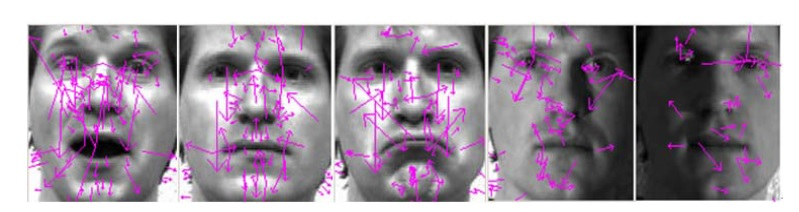
\includegraphics[width=0.8\textwidth]{Chapter2/Figs/SIFT.jpg}
  \textbf{
    \caption{An example of images with extracted SIFT features. The images represent the same object with different expression and illumination \citep{zhang2008face}}
    \label{fig:SIFT}}
\end{figure}
%%%%%%%%%%%%%%%%%%%%%%%%%%%%%%%%%%%%%%%%%%%%%%%%%%%%%%%%%%%%%%%%%


 Speeded Up Robust Features (SURF) were first presented by Herbert Bay as novel scale- and rotation-invariant interest point detectors and descriptors \citep{bay2006surf,bay2008speeded}. SURF is based on similar SIFT descriptor \citep{lowe1999object} properties.  SURF is faster than SIFT and gives as good a performance as SIFT \citep{panchal2013comparison}. (D-SURF) is a local feature detector and descriptor. It has been commonly used in computer vision tasks and object recognition classification. The D-SURF algorithm is based on the same principles and steps as SIFT, but the details in each step are different. The algorithm has three main parts: Firstly "interest point detection" was selected at important locations in the image, for an instance, at T-junctions, corners and blobs. To achieve that, the algorithm uses a very basic Hessian matrix approximation because of its good performance in accuracy \citep{bay2008speeded}.The local next step is neighbourhood description, and matching is similar to the gradient information extracted by SIFT.


\citet{uijlings2010real}

 
 




\subsubsection{Local Binary Patterns (LBP)}

Local binary patterns (LBP) method was first proposed by \citet{ojala1996comparative} as a texture descriptor depending on statistical analysis, and since then it has been widely used for face analysis due to their classification performance \citep{zhou2013local}. The LPB operator compares each pixel in a 3x3 neighbourhood of the pixel to the central value and constructs a binary digit number from the result, thus computing local texture characteristics. One of the most important advantages of LBP features is their tolerance against illumination variation\citep{shan2009facial}. Let us, therefore, define texture T in a local neighbourhood of a grayscale
image as the joint distribution of the gray levels of $P + 1 (P > 0)$ image
pixels:
%%%%%%%%%%%%%%%%%%%%%%%%%%%%%%%%%%%%%%%%%%%%%%%%%%%%%%%%%%%%%%%%%
\begin{equation}\label{eq:LBP_operator1}
T = t(g_c,g_0, ... , g_{P-1})
\end{equation}
%%%%%%%%%%%%%%%%%%%%%%%%%%%%%%%%%%%%%%%%%%%%%%%%%%%%%%%%%%%%%%%%%
where $g_c$ corresponds to the gray value of the centre pixel of a local neighbourhood. $g_p (p=0, ..., P-1)$ is the gray values of P equally spaced pixels on
a circle of radius $R (R > 0)$ that form a circularly symmetric set of neighbours.

%%%%%%%%%%%%%%%%%%%%%%%%%%%%%%%%%%%%%%%%%%%%%%%%%%%%%%%%%%%%%%%%%
 \begin{figure}[H]
\centering
  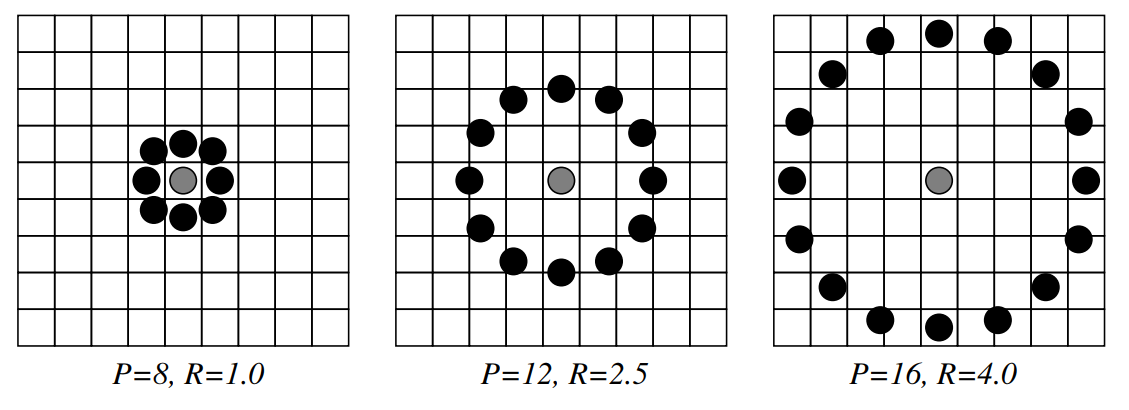
\includegraphics[width=90.5mm]{Chapter4/Figs/LBP.png}
  \textbf{\caption{Circularly symmetrical neighbour sets. Samples that do not exactly
match the pixel grid are obtained via interpolation.}\label{fig:LBP_Circularly}}
    \end{figure}
%%%%%%%%%%%%%%%%%%%%%%%%%%%%%%%%%%%%%%%%%%%%%%%%%%%%%%%%%%%%%%%%%

Figure \ref{fig:LBP_Circularly} shows three examples of different values of P and R.  To achieve invariance with respect to any monotonic transformation of the
grayscale, only the signs of the differences are considered:

%%%%%%%%%%%%%%%%%%%%%%%%%%%%%%%%%%%%%%%%%%%%%%%%%%%%%%%%%%%%%%%%%
\begin{equation}\label{eq:e joint_difference_distribution}
T = t(s(g_0 - g_c) , ... , (g_{P-1} - g_c))
\end{equation}
%%%%%%%%%%%%%%%%%%%%%%%%%%%%%%%%%%%%%%%%%%%%%%%%%%%%%%%%%%%%%%%%%

where  corresponds to the grey value of the centre pixel $(x_c, y_c)$, into the grey values of the 8 surrounding pixels, and function s(x) is defined as:

%%%%%%%%%%%%%%%%%%%%%%%%%%%%%%%%%%%%%%%%%%%%%%%%%%%%%%%%%%%%%%%%%
\begin{equation}\label{eq:LBP_operator2}
s(x) = \left\{ \begin{array}{rl}
 1 &\mbox{ if $x \geq    0$} \\
  0 &\mbox{ if $x < 0$}
       \end{array} \right.
  \end{equation}
%%%%%%%%%%%%%%%%%%%%%%%%%%%%%%%%%%%%%%%%%%%%%%%%%%%%%%%%%%%%%%%%%

The code characterizes the local image texture around (xc, yc):


%%%%%%%%%%%%%%%%%%%%%%%%%%%%%%%%%%%%%%%%%%%%%%%%%%%%%%%%%%%%%%%%%
\begin{equation}\label{eq:LBP_operator3}
LBP_{P,R}(x_c, y_c) =\sum_{p=0}^{P-1}  s(g_p  - g_c)2^n
\end{equation}
%%%%%%%%%%%%%%%%%%%%%%%%%%%%%%%%%%%%%%%%%%%%%%%%%%%%%%%%%%%%%%%%%


 
The number of neighbours used to compute the basic LBP for each pixel in the input image is 8 neighbours. Figure \ref{fig:LBPThresholdng} shows an example of LBP thresholding depending on 8 neighbours. The LBP operator is calculates the binary pattern according to equation \ref{eq:LBP_operator2}. The final decimal number calculated by the weights for each neighbour.

In LBP, the image is divided into a number of cells $n_c$ which depends on the size of each cell. For example, if we have  image $I$ ,  and apply cell size $c$, the number of cells is calculated by the following  equation:

%%%%%%%%%%%%%%%%%%%%%%%%%%%%%%%%%%%%%%%%%%%%%%%%%%%%%%%%%%%%%%%%%
\begin{equation}\label{eq:NoOfLBPCells}
n_c = floor(size(I)/c)
  \end{equation}
%%%%%%%%%%%%%%%%%%%%%%%%%%%%%%%%%%%%%%%%%%%%%%%%%%%%%%%%%%%%%%%%%



%%%%%%%%%%%%%%%%%%%%%%%%%%%%%%%%%%%%%%%%%%%%%%%%%%%%%%%%%%%%%%%%%
\begin{figure}[H]
\centering
  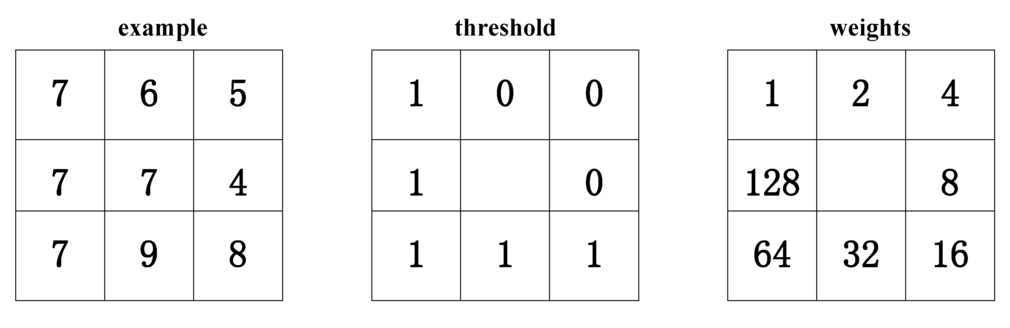
\includegraphics[width=0.42\textwidth]{Chapter4/Figs/LBPThresholdng_.png}
  \textbf{
    \caption{An example LBP thresholding depending on 8 neighbours. \\Pattern: 11110001, Decimal = 1+16+32+64+128=241.}
    \label{fig:LBPThresholdng}}
\end{figure}
%%%%%%%%%%%%%%%%%%%%%%%%%%%%%%%%%%%%%%%%%%%%%%%%%%%%%%%%%%%%%%%%%

%%%%%%%%%%%%%%%%%%%%%%%%%%%%%%%%%%%%%%%%%%%%%%%%%%%%%%%%%%%%%%%%%
\begin{figure}[H]
\centering
  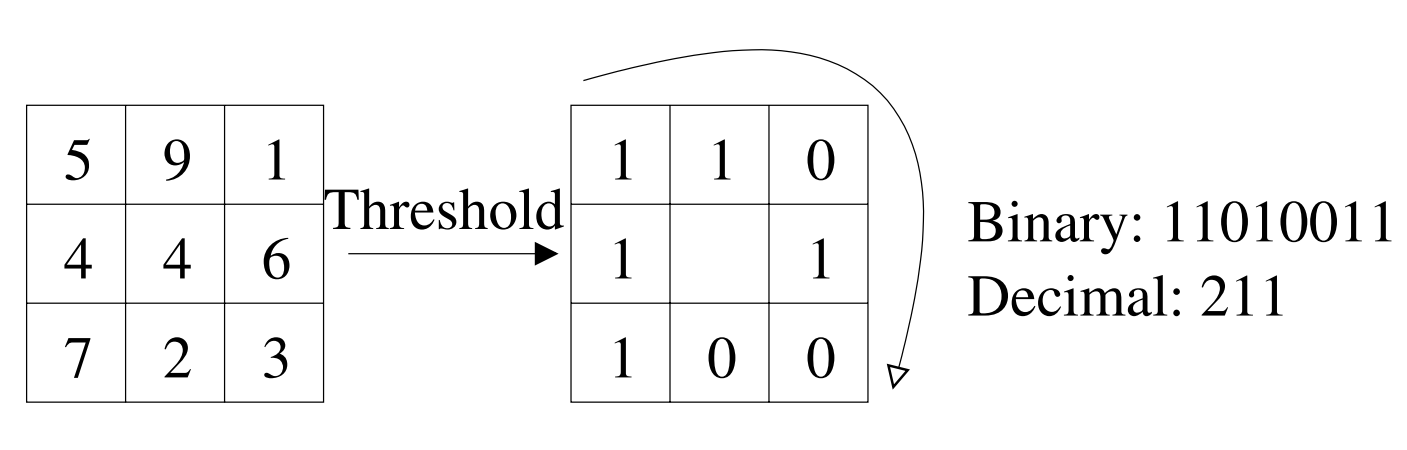
\includegraphics[width=0.7\textwidth]{Chapter2/Figs/LBPoperator.png}
  \textbf{
    \caption{The LBP operator\citep{ahonen2004face}}
    \label{fig:LBP_operator}}
\end{figure}
%%%%%%%%%%%%%%%%%%%%%%%%%%%%%%%%%%%%%%%%%%%%%%%%%%%%%%%%%%%%%%%%%


%%%%%%%%%%%%%%%%%%%%%%%%%%%%%%%%%%%%%%%%%%%%%%%%%%%%%%%%%%%%%%%%%%
%\begin{figure}[H]
%\centering
%  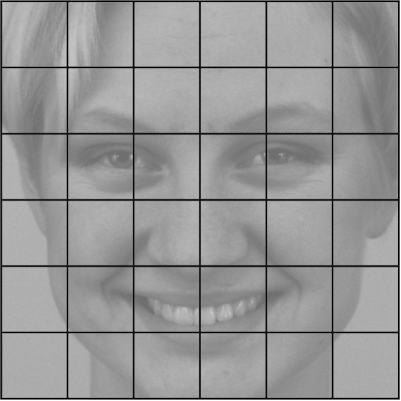
\includegraphics[width=0.25\textwidth]{Chapter4/Figs/6by6Grid.png}
%  \textbf{
%    \caption{An example of 36 cells LBP}
%    \label{fig:6by6Grid}}
%\end{figure}
%%%%%%%%%%%%%%%%%%%%%%%%%%%%%%%%%%%%%%%%%%%%%%%%%%%%%%%%%%%%%%%%%%
%


 

 LBP has been used with many classifiers to recognise facial expression because of its advantages, i.e., its tolerance of monotonic illumination changes and its computational simplicity \citep{huang2011local}. \citet{shan2005robust} used a simple Local Binary Patterns (LBP) with Support Vector Machine are (SVM). They have tested the extracted LBP features with linear, polynomial and RBF kernels SVM to classify seven facial expressions. They used the Cohn Kanade Facial Expression Database which was produced by \citet{kanade2000comprehensive}, and contains faces of 100 university student from age 18 to 30 years. \citet{shan2005robust} compared their results with Gabor wavelets, and they have found that LBP with SVM gave better classification accuracy than Gabor wavelets, and saved computational resources. They also proved that LBP give good results with different resolutions, even low-resolution images\citep{shan2005robust}. In the same area, \cite{shan2009facial} have done a comprehensive study for facial expression recognition methods based on Local Binary Patterns, and they found that LBP features are effective and efficient for facial expression recognition and it give good results with low-resolution images.
 
LBP has been used for frontal faces and for angle pose faces, \citep{moore2011local} proposed a multi-view facial expression recognition method using  some extensions including multi-scale local binary patterns ($LBP^{ms}$) and local gabor binary patterns ($LGBP$), and they have tested it on photos from multiple dataset \citep{gross2010multi} to see how see how head pose affects facial expression with SVM classifier. 

During the last decade, researchers have prosed many methods to use LBP and LBP's extensions. Some of them have tried to divide the face into equal blocks into grids \citep{moore2011local}; others have tried to divide the face into its main parts: eyes, nose and mouth as in \citet{khan2013framework} who have proposed pyramidal local binary pattern (PLBP) operator to recognise six facial expressions. They have tested the extracted features with four classifiers: nearest neighbours (2NN), Random forest (RF), SVM and decision tree. They used in experiments two datasets: CK+ and FG-NET.  






\section{Classification}
\label{sec:ch1_Classification}
In this thesis we will use two popular data classification methods, random forests (RF) \citep{breiman2001random} and support vector machine (SVM) \citep{cortes1995support}. An RF model uses the bootstrap method to build $n_{tree}$ randomly, then they are provided with randomly selected
 samples of the training input. The trees will work together to give the final decision by combining them together in a forest. SVM aims to find a hyperplane (linear decision surface) which divides data into two classes and has the largest distance between the closest elements of the two classes to each other. These elements are called vector machines. It is not easy always to find a linear decision surface, so the radial basis function (RBF) is used 
as a kernel after the data has been mapped into a higher dimensional space \citep{davison2014micro}.

\subsection{Random forest}

Random Forest (RF) is a popular method in computer vision because of its capacity to operate with  large multi-class datasets and give high accuracy results \citep{fanelli2011real}. Because of its great generalization ability, it is very fast to train and parallelise \citep{breiman2001random,belle2008detection}. RF classifier contains a combination of tree classifiers, and each one is created by a random vector independently from the input vector. Each tree gives a unit vote for the most popular class to classify an input vector \citep{breiman1999}.

To understand Random the forest algorithm, we need to understand the basic idea of decision trees. Considering an input feature $X$ and an output $Y$, we need to train a model to predict $Y$ for given feature $X$. Decision trees are  based on performing predictions using a sequence of simple decisions by an ensemble of hierarchical binary decisions \citep{Random2012Medical}. In while the decision tree,  the top node is called root connected with two children nodes, nodes at the bottom are called leaves, as shown in figure \ref{fig:decisionTree}.    

%%%%%%%%%%%%%%%%%%%%%%%%%%%%%%%%%%%%%%%%%%%%%%%%%%%%%%%%%%%%%%%%%
\begin{figure}[H]
\centering
  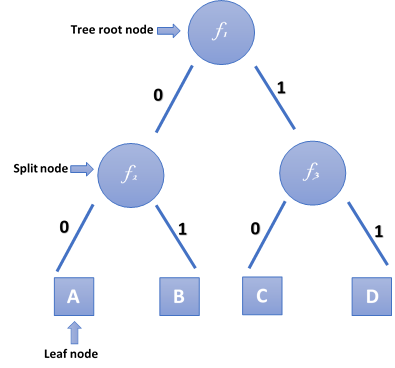
\includegraphics[width=0.4\textwidth]{Chapter2/Figs/decisionTree.png}
  \textbf{
    \caption{Simple decision tree}
    \label{fig:decisionTree}}
\end{figure}
%%%%%%%%%%%%%%%%%%%%%%%%%%%%%%%%%%%%%%%%%%%%%%%%%%%%%%%%%%%%%%%%%

The main idea of Random forest \citep{breiman2001random} $\mathcal{F}$ is to make a group (ensemble) of $T$ decision trees work together  $\mathcal{F} = \{ \mathbf{T_1}, ... ,\mathbf{T_t},...\mathbf{T_T} \}$, where each tree node in random forests classifier is a weak classifier, each tree gets a "vote" in classifying \citep{breiman1996bagging,breiman1999,breiman2001random}. This combination of ensemble  decorrelated trees provides very good generalization. So, from the same dataset, many random samples can be generated to be processed by constructing decorrelated trees.  According to \citet{breiman2001random} randomization method "Bagging",  for given dataset $\mathbf{D} = \{ \mathbf{X}^{(n)}, Y^{(n)} \}_{n=1} ^ N$ is divided into random smaller dataset. Each data set $S_t$ called bootstrap. By growing a tree $\mathbf{T_t}$ for each bootstrap, an ensemble decision trees working together to make vote for a new unseen observation.  

%%%%%%%%%%%%%%%%%%%%%%%%%%%%%%%%%%%%%%%%%%%%%%%%%%%%%%%%%%%%%%%%%
\begin{figure}[H]
\centering
  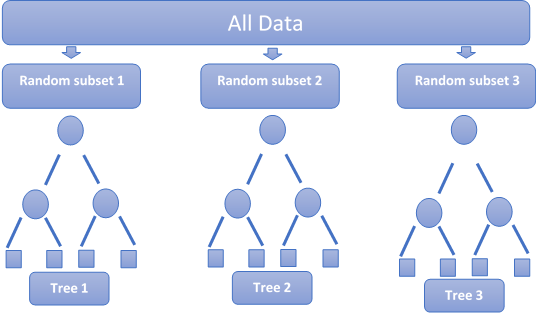
\includegraphics[width=0.50\textwidth]{Chapter2/Figs/RandomForest.png}
  \textbf{
    \caption{New subsets Randomisation by bagging method}
    \label{fig:RandomForest}}
\end{figure}
%%%%%%%%%%%%%%%%%%%%%%%%%%%%%%%%%%%%%%%%%%%%%%%%%%%%%%%%%%%%%%%%


In classification supervised training tasks, we have training data contains features and labels (output). Let given training dataset  $\{( \mathbf{X^{(n)}}, Y^{(n)}) \} _{n=1} ^N \in  \mathcal{X}  \times \mathcal{Y}$, where $\mathbf{X} \subset \mathcal{X}$ and $\mathbf{Y} \subset \mathcal{Y}$, for $\mathcal{X} \subset  \mathbb{R}^D$ the features space and the output space  $\mathcal{Y} \subset  \mathbb{R}$, which is a finite set of $K$ discrete values $\mathcal{Y} = \{y_1,...,y_k,...,y_K\}$  represent the the classes . Let us consider the partition $\mathcal{P}_t =\{ \mathcal{C}_t^{(zt)} \}  _{z_t=1} ^{Z_t}$ built by the random tree  $\mathbf{T}_t$ \citep{Random2012Medical}. Class posteriors can be simply approximated in each cell $\mathcal{C} ^{(zt)}$ of $\mathcal{P}_t$ as follows:

%%%%%%%%%%%%%%%%%%%%%%%%%%%%%%%%%%%%%%%%%%%%%%%%%%%%%%%%%%%%%%%%%
\begin{equation}\label{eq:cell_posteriori}
P(y_k \mid \mathbf{X} \in \mathcal{C}_t ^ {(z_t)} ,  \mathcal{P}_t) = \frac{\mid \{ \mathbf{X}^{(n)} \in \mathcal{C}_t ^ (z_t), Y^{(n)} = y_k \} \mid } {\mid \{  \mathbf{X}^{(n)} \in \mathcal{C}_t ^ {(z_t)} \} \mid }
\end{equation}
%%%%%%%%%%%%%%%%%%%%%%%%%%%%%%%%%%%%%%%%%%%%%%%%%%%%%%%%%%%%%%%%




In classification tasks, if a trained model is given a new unseen feature and it should  predict to which class does it  refer by sending the unseen feature through all trees of the forest and combining tree posteriors.   class prediction for a new observation is the class that yields the largest weighted average of the class posterior probabilities computed using selected trees only.  For each class $c \in \mathcal{C}$ and each tree $t=1, ... ,T$. Prediction for new observation $x$ computes $\hat{P}(c\mid x)$ to estimate posterior probability of class $c$ using $t$. $\mathcal{C}$ is the set of all distinct classes in the training data:

%%%%%%%%%%%%%%%%%%%%%%%%%%%%%%%%%%%%%%%%%%%%%%%%%%%%%%%%%%%%%%%%%
\begin{equation}\label{eq:maximum_posteriori}
\hat{P}_{bag}= \frac{1}{\sum_{t=1}^{T} \alpha_t I(t\in S)} \sum_{t=1}^{T} \alpha_t \hat{y_t} I(t\in S)
\end{equation}
%%%%%%%%%%%%%%%%%%%%%%%%%%%%%%%%%%%%%%%%%%%%%%%%%%%%%%%%%%%%%%%%
where $\hat{y_t}$ is the prediction from tree t in the ensemble, $S$ is the set of indices of selected trees that comprise the prediction and $\alpha_t$ is the weight of the tree.


%%%%%%%%%%%%%%%%%%%%%%%%%%%%%%%%%%%%%%%%%%%%%%%%%%%%%%%%%%%%%%%%%
\begin{equation}\label{eq:maximum_posteriori}
\hat{Y}_{bag}= argmax_{c \in \mathcal{C}} \{ P_{bag}(c \mid x)\}
\end{equation}.
%%%%%%%%%%%%%%%%%%%%%%%%%%%%%%%%%%%%%%%%%%%%%%%%%%%%%%%%%%%%%%%%



 


The RFs classifier has proficient power to gauge the importance of each features variable (predictor) \citep{breiman2001random} by calculating how much a prediction error increases or decrease  when (OOB) data for that variable is permuted while all others are passed on unaltered. The computations are carried out tree by tree as the random forest is built \citep{breiman2001random,breiman2002manual,liaw2002classification}.


Breiman has proposed a method to evaluate the variable importance by measuring the Mean Decrease Accuracy of the forest when the values of $X_m$ are randomly permuted in the out-of-bag samples. Suppose we have M input variables. After each tree is built, the values of the $m_{th}$ variable in the out-of-bag examples are randomly permuted, and the out-of-bag data is run down the corresponding tree. The classification given for each $x_n$ that is out of the bag is saved. This is repeated for $m=1,2, ... , M$. At the end of the run, the plurality of out-of-bag class votes for $x_n$ with the $m_th$ variable noised up is compared with the true class label of $x_n$ to give a misclassification rate. The output is the percent increase in misclassification rate as compared to the out-of-bag rate (with all variables intact).\citep{breiman2001random,louppe2013understanding}.


In classification problems, (OOB) error returns the weighted misclassification rate.

oobError predicts classes for all out-of-bag observations.

The weighted misclassification rate estimate depends on the value of 'Mode'.
If you specify 'Mode','Individual', then oobError sets any in bag observations within a selected tree to the predicted, weighted, most popular class overall training responses. If there are multiple most popular classes, error considers the one listed first in the Class Names property of the TreeBagger model the most popular. Then, oobError computes the weighted misclassification rate for each selected tree.

If you specify 'Mode','Cumulative', then ooError returns a vector of cumulative, weighted misclassification rates, where et* is the cumulative, weighted misclassification rate for selected tree t. To compute et*, for each observation that is out of the bag for at least one tree through tree t, oobError finds the predicted, cumulative, weighted most popular class through tree t. oobError sets observations that are in the bag for all selected trees through tree t to the weighted, most popular class overall training responses. If there are multiple most popular classes, error considers the one listed first in the ClassNames property of the TreeBagger model the most popular. Then, oobError computes et*.


If you specify 'Mode','Ensemble', then, for each observation that is out of the bag for at least one tree, oobError computes the weighted, most popular class over all selected trees. oobError sets observations that are in bag for all selected trees through tree t to the predicted, weighted, most popular class overall training responses. If there are multiple most popular classes, error considers the one listed first in the Class Names property of the TreeBagger model the most popular. Then, oobError computes the weighted misclassification rate , which is the same as the final, cumulative, weighted misclassification rate.

\subsection{Support Vector Machine (SVM)}
SVM is a binary classifier, and it was first proposed by Vladimir Vapnik in 1979 and first published in 1995. The basic idea of SVM is to find the hyperplane that linearly separates the n-dimensional data into two classes. Data do not always accept linear separating,  so  \citet{hsu2003practical} suggested to use four essential kernel functions, Linear, Polynomial, Radial Basis Function (RBF)and sigmoid. SVM training aims to build a model from training data to be able to predict new values in testing data \cite{candra2017emotion}.
So if we have labelled training data $(x_i,y_i),..., i =1$ where $x_i \in R_n$ and $y \in \{1,-1\}$ the SVM seeks to find a solution of the optimisation problem:
\begin{equation}
\min_{w,b,\xi} \frac{1}{2} w^T w + C \sum_{i=1}^{l} \xi
\end{equation} 

is subject to

\begin{equation}
y_i(w^T  \phi(x_i) + b) \geq 1 \xi_{i},  \xi_{i} \geq, i = 1,... ,l 
%(w^T + b) \geq 1 − _i,
\end{equation} 
\newpage

SVM aims to find a linear separating hyperplane with the maximal margin in the training data space. Hsu et al. suggested to use four basic kernels for higher dimensional space: linear, polynomial, sigmoid and Radial Basis Function (RBF).
 In this thesis, the SVM classifier is optimised using an RBF kernel by Bayesian optimization method which is a powerful method to optimise functions \citep{mockus2012bayesian}. 
\begin{equation}
K(x_i, x_j)  = exp(-\gamma  \parallel x_i - x_j \parallel ^ 2),\gamma > 0
\end{equation}
 

%\section{Optimisation}
%Optimisation methods try to find the optimal values which
%maximising or minimising a function, often representing a range of choices available in a particular situation, by performing a  comparison of the different options for determining which might be the optimal values. In machine learning, classifiers such as SVM need to determine the best parameters to optimise the accuracy and avoid misclassification. In this section, I will explain the main ideas behind three optimisation methods: Nelder-Mead simplex direct search, Bayesian optimization method and Covariance Matrix Adaptation Evolution Strategy.   
%\subsection{Nelder-Mead simplex direct search}
%
%The Nelder–Mead method or (downhill simplex method)  is a common method used to determine the maximum or minimum of a function in a multidimensional space \cite{nelder1965simplex}.
%
%If we are trying to minimize the function ${\displaystyle f(\mathbf {x} )})$, where ${\displaystyle \mathbf {x} \in {\mathbb {R} }^{n}} {\displaystyle \mathbf {x} \in {\mathbb {R}}^{n}}$. Our current test points are ${\displaystyle \mathbf {x} _{1},\ldots ,\mathbf {x} _{n+1}} {\displaystyle \mathbf {x} _{1},\ldots ,\mathbf {x} _{n+1}}$
%
%\begin{enumerate}
%
%\item \textbf{Order according to the values at the vertices:}
%
%${\displaystyle f(\mathbf {x} _{1})\leq f(\mathbf {x} _{2})\leq \cdots \leq f(\mathbf {x} _{n+1})}$.
%
%
%Check if method should stop. See Termination below. Sometimes inappropriately called "convergence".
%
%\item \textbf{Calculate ${\displaystyle \mathbf {x} _{o}}$, the centroid of all points except ${\displaystyle \mathbf {x} _{n+1}}$.}
%
%\item \textbf{Reflection}
%
%Compute reflected point ${\displaystyle \mathbf {x} _{r}=\mathbf {x} _{o}+\alpha (\mathbf {x} _{o}-\mathbf {x} _{n+1})}$ with ${\displaystyle \alpha >0} $.
%
%If the reflected point is better than the second worst, but not better than the best, i.e $ {\displaystyle f(\mathbf {x} _{1})\leq f(\mathbf {x} _{r})<f(\mathbf {x} _{n})}$,
%then obtain a new simplex by replacing the worst point ${\displaystyle \mathbf {x} _{n+1}}$ with the reflected point ${\displaystyle \mathbf {x} _{r}} $, and go to step 1.
%
%\item \textbf{Expansion}
%
%If the reflected point is the best point so far, ${\displaystyle f(\mathbf {x} _{r})<f(\mathbf {x} _{1})}$ ,
%then compute the expanded point ${\displaystyle \mathbf {x} _{e}=\mathbf {x} _{o}+\gamma (\mathbf {x} _{r}-\mathbf {x} _{o})}$  with ${\displaystyle \gamma >1} \gamma >1$.
%If the expanded point is better than the reflected point, ${\displaystyle f(\mathbf {x} _{e})<f(\mathbf {x} _{r})}$ ,
%then obtain a new simplex by replacing the worst point ${\displaystyle \mathbf {x} _{n+1}}$  with the expanded point ${\displaystyle \mathbf {x} _{e}}$ ${\displaystyle \mathbf {x} _{e}} and go to step 1$;
%else obtain a new simplex by replacing the worst point ${\displaystyle \mathbf {x} _{n+1}}$ with the reflected point ${\displaystyle \mathbf {x} _{r}}$  and go to step 1.
%
%
%\item \textbf{Contraction}
%
%Here it is certain that ${\displaystyle f(\mathbf {x} _{r})\geq f(\mathbf {x} _{n})}$. (Note that ${\displaystyle \mathbf {x} _{n}}$  is second or "next" to highest.)
%Compute contracted point ${\displaystyle \mathbf {x} _{c}=\mathbf {x} _{o}+\rho (\mathbf {x} _{n+1}-\mathbf {x} _{o})}$  with ${\displaystyle 0<\rho \leq 0.5}$.
%If the contracted point is better than the worst point, i.e. ${\displaystyle f(\mathbf {x} _{c})<f(\mathbf {x} _{n+1})}$,
%then obtain a new simplex by replacing the worst point ${\displaystyle \mathbf {x} _{n+1}}$  with the contracted point ${\displaystyle \mathbf {x} _{c}}$  and go to step 1;
%
%\item \textbf{Shrink}
%
%Replace all points except the best (${\displaystyle \mathbf {x} _{1}}$) with
%${\displaystyle \mathbf {x} _{i}=\mathbf {x} _{1}+\sigma (\mathbf {x} _{i}-\mathbf {x} _{1})}$  and go to step 1.
%
%\end{enumerate}
%
%\subsection{Bayesian optimization method}
%
%\subsection{Covariance Matrix Adaptation Evolution Strategy}
%Covariance Matrix Adaptation Evolution Strategy (CMA-ES) is a derivative-free method for numerical optimization of non-linear or non-convex continuous optimization problems, ans it belong to the class of evolutionary algorithms and evolutionary computation. 



\section{Summary}
\label{sec:ch1_Summary}

In this chapter, we have reviewed some of the basic concepts regarding facial expression recognition and related topics such as 
features extraction and classification necessary to appreciate our proposed facial expression recognition method.
We talked about the background of facial analysis, and we briefly introduced currents techniques which might be useful for our thesis. 